\section{Discussion}
\label{sec:discussion}

We hypothesized that neural networks might exhibit biases in their ability to learn distance versus intensity representations. However, the results reveal surprising and counterintuitive behaviors. ReLU2, which is constrained to learn an intensity representation, failed catastrophicaly. Abs2-Neg designed to enforce distance representations, underperformed compared to Abs2, its intensity-learning counterpart. We explore possible reasons for these conflicting results.

We initially hypothesized that neural networks would exhibit a preference for learning distance-based representations over intensity-based ones. However, the results reveal surprising and counterintuitive behaviors. While ReLU2, constrained to learn an intensity representation, failed catastrophically, and Abs2-Neg, designed to enforce distance representations, underperformed compared to its intensity counterpart, Abs2 exhibited surprising resilience under intensity constraints. We explore possible reasons for these conflicting results.

\subsection{Feature Distributions in Latent Spaces}

To investigate the network's internal processes, we analyze the distance distributions of data points from the hyperplanes defined by the nodes of the first linear layer. This distance corresponds to the preactivation values and geometrically represents how far each input lies from a decision boundary. Since we do not have direct access to the exact features learned by each node, we use MNIST class labels as proxies for these features. While this approach assumes that each class captures distinct, meaningful aspects of the data, it allows us to gain insights into the network's behavior at a granular level.

Figure~\ref{fig:distance_distribution} shows an example of these class distributions. Each histogram reveals a cluster of points corresponding to a specific class, exhibiting heterogeneity in statistical properties such as mean, variance, skewness, and modality. Class distributions overlap significantly, and the extent of this overlap varies across nodes. The specific class overlaps vary depending on the linear projection. This isn't surprising and is what we expect for data that is not directly linearly separable.

\begin{figure}[H]
    \centering
    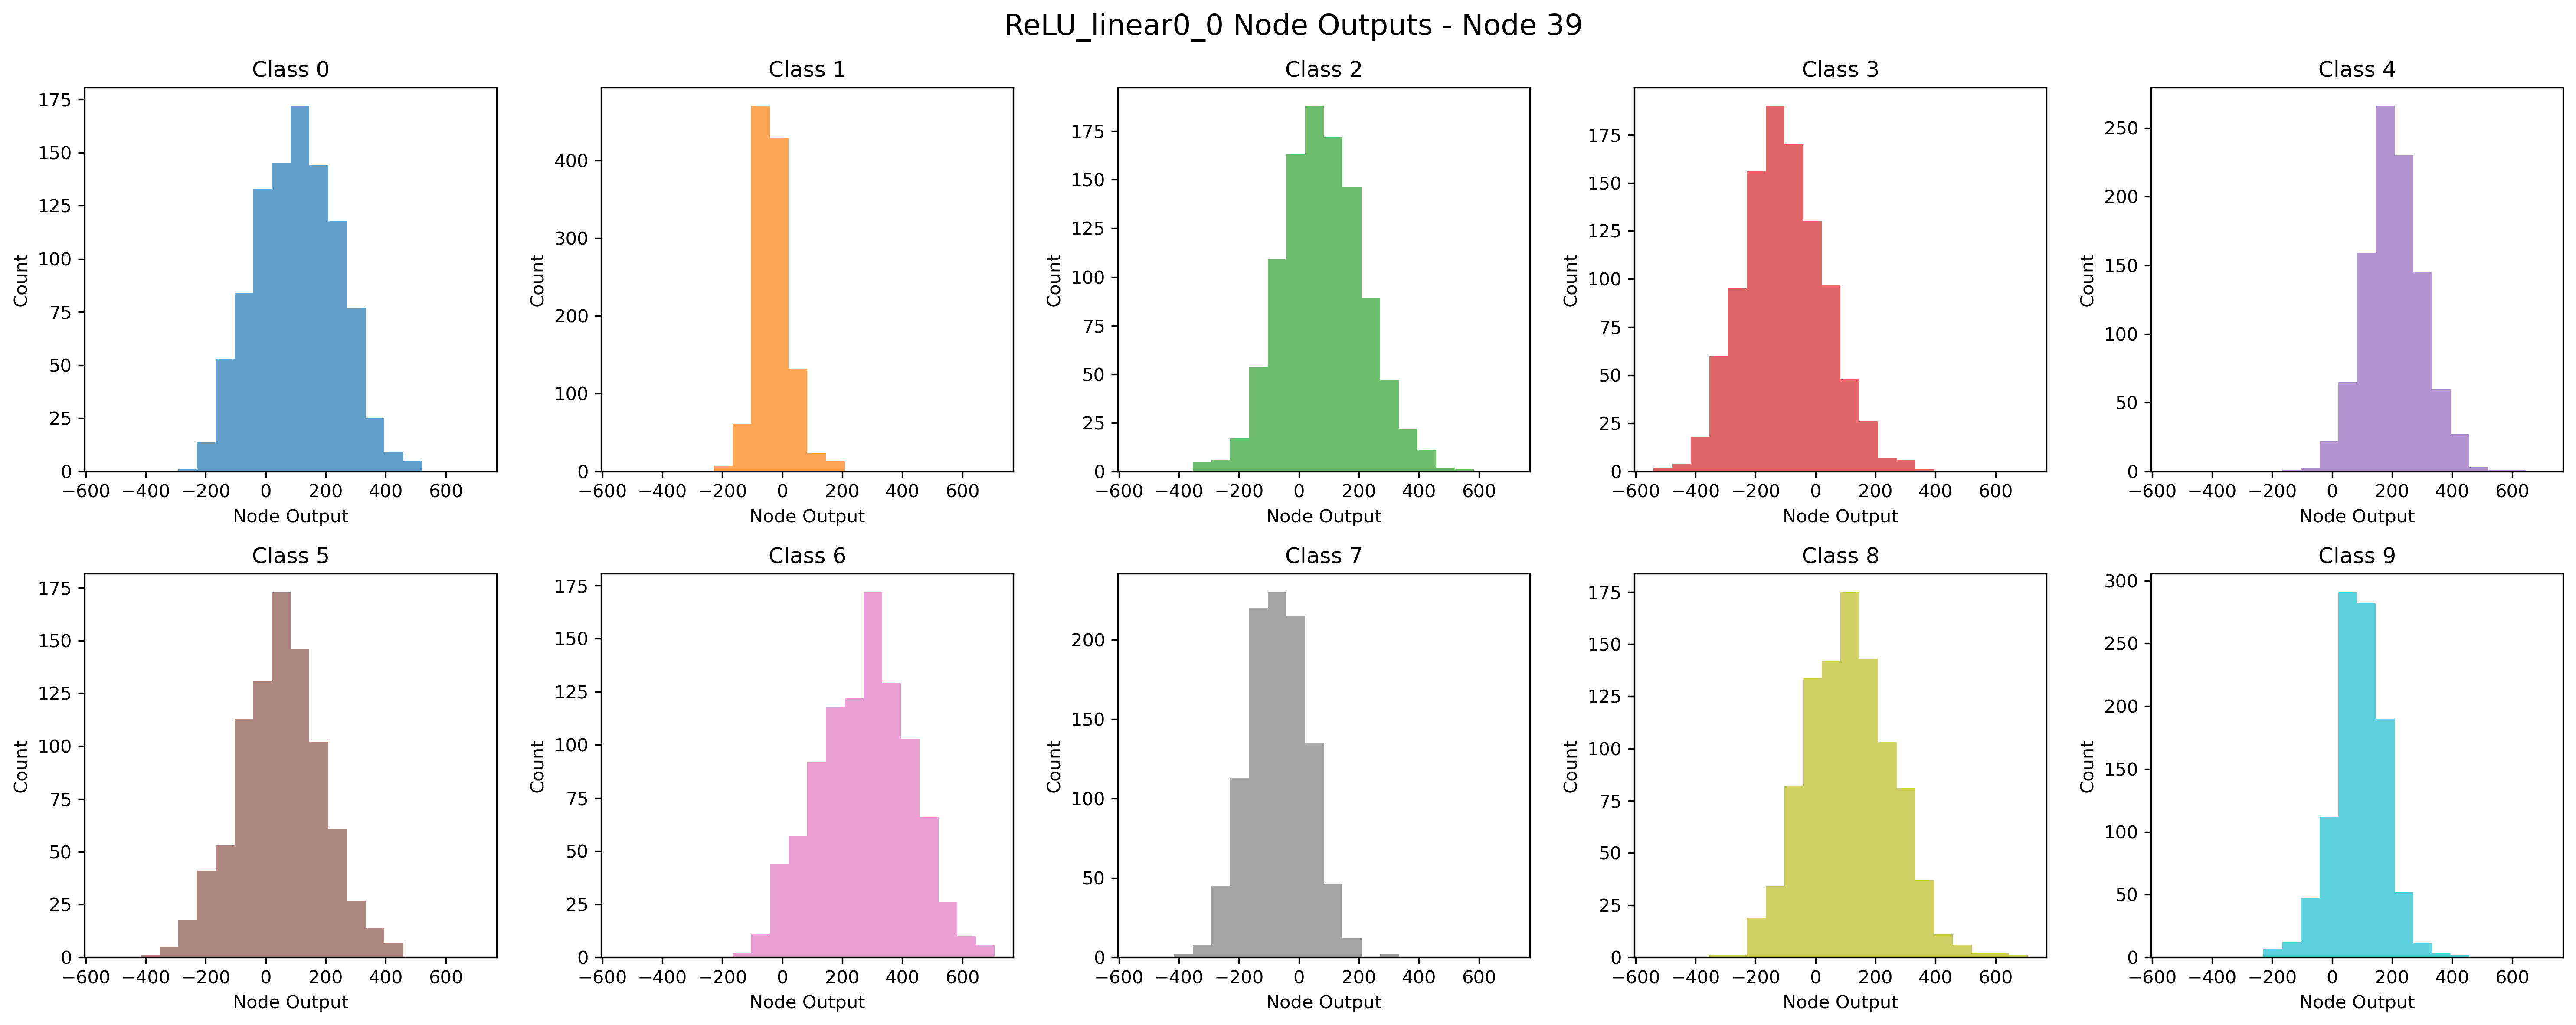
\includegraphics[width=0.4\textwidth]{images/distance_distribution}
    \caption{An example of class distributions. Each histogram reveals a cluster of points corresponding to a specific class, exhibiting heterogeneity in statistical properties such as mean, variance, skewness, and modality.}
    \label{fig:distance_distribution}
\end{figure}

Together, all of the outputs of the first linear layer form a 128-dimensional latent space. The second linear layer defines a 128-dimensional hyperplane $y=Wx+b$ in 129-dimensional space, where the scalar output $y$ extends the original 128 dimensions and $b=0$. While most analyses of linear layers focus on linear separation, we can also interpret a hyperplane by examining the specific points it intersects within the latent space. These points of intersection can be interpreted as representing prototypes or characteristic features learned by the network, as discussed in Section~\ref{sec:background}. The hyperplane defined by the second linear layer can be uniquely defined by 128 linearly independent points. Crucially, 127 of these points lie on the decision boundary *within* the 128-dimensional latent space, representing the learned prototypes. The origin is one of the prototype points because of the lack of bias. The final point exists in the 129-dimensional space $(x,y \neq 0)$ *outside* of the latent space and does not directly contribute to defining the prototypes. This means that the location and orientation of the hyperplane *within the latent space* are completely determined by the 126 learned points on the decision boundary, and any change to these points would result in a different hyperplane. The second linear layer, therefore, acts as a mechanism for combining these prototype representations to produce the final classification output.

We can imagine an ideal point $z_c$ in the 128-dimensional latent space that represents an optimal "center" of class $c$. Each dimension of this latent space corresponds to the output of a single node in the first linear layer. For each class, we consider an optimal $z_c$ that minimizes the average distance to points belonging to class $c$ while maximizing the average distance to points belonging to other classes. Conversely, we consider a point $z_{\neg c}$ that does the opposite, maximizing the average distance to class $c$ while minimizing the average distance to other classes.

When the second linear layer is learning a distance representation, it is attempting to define a 128-dimensional hyperplane that laerns to intersects 126 linearly independent points on the decision boundary within the latent space that approximate $z_c$. This positioning allows the hyperplane to effectively separate classes based on proximity to their respective ideal centers, resulting in the target class having the smallest activation average across the latent space dimensions.

When learning an intensity representation, the second linear layer is attempting to define a hyperplane that learns to intersects 126 linearly independent points on the decision boundary within the latent space that approximate $z_{\neg c}$. This positioning effectively separates classes based on their distance from the target "anti-centers" -- the centers of non-target classes -- resulting in the non-target classes having smaller average activations, and thus the target class having the largest activation average across latent space dimensions.

\subsection{Analysis of ReLU-based Architectures}

The catastrophic failure of \texttt{ReLU2} ($47.20\% \pm 12.00\%$) underscores the inherent brittleness of this architecture under intensity-based constraints. Analysis of activation patterns on the test set revealed a significant prevalence of dead nodes in the output layer (\texttt{activation1}), with $33.00\%$ permanently inactive (never outputting a positive value) and an additional $53.50\%$ rarely active (outputting a positive value for less than 5\% of inputs). In contrast, none of the other models had dead or rarely used nodes in their output layers. We theorize this pattern emerges because the network is learning a disjunctive distance representation, where smaller activations for non-target classes often place them on the negative side of the decision boundary. Since each digit class represents only 10\% of the dataset, approximately 90\% of the samples belong to non-target classes for any given classification decision, potentially leading to a large number of negative pre-activations that are subsequently zeroed out by the second ReLU.

The mechanism behind this dead node collapse can be understood in the context of the network's attempt to minimize the activations for non-target classes $\neg c$ when constructing a disjunctive distance representation. If the target class is not linearly separable in these individual node outputs, the optimization process, as it minimizes $\neg c$, inadvertently minimizes the activations for the overlapping class $c$ as well. The 9:1 imbalance between $\neg c:c$ exacerbates this process. This results in a situation where inputs from both the target and non-target classes produce negative pre-activations, leading to widespread node inactivity after the second ReLU is applied in \texttt{ReLU2}. This collapse towards the negative side, driven by the intensity-based constraint of the second ReLU, produces the observed prevalence of dead nodes.

In contrast, \texttt{ReLU2-Neg} achieved near-baseline performance ($94.93\% \pm 0.15\%$). In this architecture, the second linear layer builds a conjunctive distance representation by minimizing activation values for points of class $c$. Since $z_c$ represents the center of class $c$'s distribution across the latent space, this positioning ensures most points from class $c$ have negative pre-activation values. The ReLU converts the negative values to zero. It also zeroes out the classes with a pre-activation less than the target class (to the left of the target in the distance histogram Figure~\ref{fig:distance_distribution}. Under ReLU each hyperplane learns a set of features, indicated by the zero activation. As long as those features are uncorrelated with the target across the hyperplanes, the target class still exhibits the smallest activation. The diverse projections that create the latent space ensure this decorrelation. This positioning effectively minimizes the target class $c$ while maximizing $\neg c$.

\subsection{Analysis of Abs-based Architectures}

Abs networks differ from ReLU in that they cannot produce dead nodes. Instead of zeroing out negative values, Abs folds them back to the positive side, ensuring all nodes remain active. Under our distance metric theory, where zero activation indicates maximum feature membership, this architectural difference leads to distinct behaviors in how features are represented. In ReLU networks, maximum feature membership extends to all points in the region of the input space that produces negative pre-activation values, creating larger feature sets. In contrast, Abs networks achieve maximum feature membership only at points exactly on the decision boundary, resulting in more focused feature sets. Since this minimum value can correspond to either $z_c$ or $z_{\neg c}$, the learned representation becomes easier to interpret because it directly reflects the distances to the learned prototypes or anti-prototypes.

While \texttt{Abs2} achieved strong performance ($95.35\% \pm 0.17\%$), its counterpart designed to learn distance representations, \texttt{Abs2-Neg}, showed significantly degraded accuracy ($90.08\% \pm 2.56\%$), with notably higher variance and a performance gap of over $5$ percentage points. What factors contribute to this surprising performance discrepancy between \texttt{Abs2} and \texttt{Abs2-Neg}?

We theorize the \texttt{Abs2} hyperplane is positioned such that $z_{\neg c}$, the centers of non-target classes, lie on the decision boundary, and the \texttt{Abs2-Neg} hyperplane is positioned such that $z_c$, the center of the target class, lies on the decision boundary. Unlike with \texttt{ReLU}, \texttt{Abs2-Neg} can actually place $z_c$ on the hyperplane and fold the values around it due to the absolute value operation, resulting in larger positive values for points farther from $z_c$. While both architectures learn sets of classes when there is class overlap, \texttt{Abs2-Neg} constructs a *conjunctive* representation, focusing on the target class. This results in smaller, more specific class sets compared to those learned by \texttt{ReLU2}, which constructs a *disjunctive* representation.

We theorize that Abs2-Neg performs worse because, due to the strong clustered nature of MNIST, there is a single optimal $z_c$. The Abs2-Neg hyperplane must intersect this optimal point and 127 additional linearly independent points to be fully defined. Since there is only one optimal $z_c$ that best separates each target class from all others, these additional points must necessarily be non-optimal separation points. These non-optimal points introduce false positives on for the target class and false negatives for the non-target classes. 

We theorize that \texttt{Abs2-Neg} performs worse because, due to the strongly clustered nature of MNIST, where each digit class tends to occupy a relatively distinct region of the input space, there is a single optimal $z_c$ that best separates each target class from all others. The \texttt{Abs2-Neg} hyperplane must intersect this optimal point and 127 additional linearly independent points to be fully defined. Since there is only one optimal $z_c$, these additional points must necessarily be non-optimal separation points. These points, by definition, lie farther from the ideal center of the target class and closer to the non-target classes. Consequently, the hyperplane, constrained to pass through these non-optimal points, will inevitably misclassify some data points, leading to false positives for the target class and false negatives for the non-target classes. 

\texttt{Abs2}, on the other hand, must select $z_{\neg c}$ for each dimension $i$ of the latent space. For each dimension, it can choose any of the nine non-target classes to place $z_{\neg c}[i]$, with each choice potentially creating a useful decision boundary for separating the target class from that specific non-target class. With nine choices for each of the 128 dimensions ($9^{128}$ possible combinations), \texttt{Abs2} has an enormous space of potential solutions when selecting its hyperplane points. This combinatorial flexibility in selecting points allows \texttt{Abs2} to position its hyperplane such that it achieves effective separation of target classes even when individual points are not optimal, as it can compensate for suboptimal choices in some dimensions by making better choices in others.

\subsection{Validation Through Additional Experiments}

Our theory about the \texttt{Abs2-Neg} performance drop suggests that a layer designed to explicitly represent the distance to a single optimal point might correct the performance difference. If our hypothesis is correct, explicitly incorporating this geometric constraint into the architecture should improve performance. We can achieve this by designing a layer, which we call OffsetL2, that computes the weighted L2 distance from a learned reference point $\mu$. The L2 distance is a natural choice for representing Euclidean distance and is easily differentiable, making it suitable for gradient-based optimization. Specifically, we propose a layer that computes:

$y_i = || \alpha_i \odot (x - \mu_i) ||_2$

where $x$ is the input vector, $\mu_i$ represents the hypothesized optimal point $z_c$ for output $i$, $\alpha_i$ is a weight vector  that allows the network take a weighted L2-norm of the offset latent space. $\mu_i$ and $\alpha_i$ are both learned through backpropagation and are the same size as the input. Element-wise multiplication, denoted with $\odot$, also outputs a vector shaped like the input. The L2-norm is calculated over the elements of that vector. Each output node $i$ has its own corresponding values $\mu_i$ and $\alpha_i$. This formulation directly embeds our geometric intuition: rather than implicitly discovering optimal points through hyperplane positioning as in \texttt{Abs2-Neg}, the OffsetL2 layer explicitly learns a single reference point, $\mu_i$, for each output $i$ and measures the Euclidean distance from it.

We refer to this architecture as OffsetL2. While \texttt{Abs2-Neg} must construct its hyperplane through $z_c$ and 127 additional points that may not be optimal for class separation, OffsetL2 directly optimizes a single prototype $\mu$, intended to represent the optimal distance point $z_c$, and its associated importance weights $\alpha$. This design eliminates the need for the network to discover implicit geometric relationships through hyperplane positioning, instead allowing it to learn an explicit optimal reference point for each class. The $\alpha$ weights provide flexibility, similar to \texttt{Abs2}'s ability to emphasize different input dimensions, but do so through direct scaling, allowing it to learn which dimensions are most relevant for determining the distance to the optimal point for each class. Therefore, OffsetL2 offers a more direct and potentially more effective way to learn distance-based representations compared to the implicit hyperplane positioning of \texttt{Abs2-Neg}.

We expect this architecture to perform well for both distance and intensity learning, since it can learn either the optimal $z_c$ or $z_{\neg c}$ as its prototype. The flexibility provided by $\alpha$ allows the network to appropriately weight the dimensions of the latent space regardless of which reference point is being learned. When we incorporate OffsetL2 into the \texttt{Abs2-Neg} model and combine it with the LogSoftmax function used in CrossEntropyLoss, the resulting architecture bears a striking resemblance to Radial Basis Function (RBF) networks. The key equations highlight this similarity: 

We expect this architecture to perform well for both distance and intensity learning, since it can learn either the optimal $z_c$ or $z_{\neg c}$ as its prototype. The flexibility provided by $\alpha$ allows the network to appropriately weight the dimensions of the latent space regardless of which reference point is being learned. When we incorporate OffsetL2 into the \texttt{Abs2-Neg} model and combine it with the LogSoftmax function used in CrossEntropyLoss, the resulting architecture bears a striking resemblance to Radial Basis Function (RBF) networks and to the Mahalanobis distance, as described in Section~\ref{sec:background}. The key equations highlight this similarity:

    \text{OffsetL2 + LogSoftmax:}

    $y_i = \exp(- || \alpha_i \odot (x - \mu_i) ||_2 )$

    \text{Traditional RBF:}
    
    $y_i = \exp( -0.5(precision_i (x - \mu_i)^2) )$

    \text{Gaussian PCA Mahalanobis Distance + LogSoftmax:}
    
    $y_i = \exp( -||(precision_i v_i (x - \mu_i)||_2) )$


The primary distinction from RBF lies in our inclusion of the learnable weight vector $\alpha_i$, which allows the network to modulate the importance of different dimensions in computing the distance from the prototype.  When OffsetL2 is preceded by a linear layer, it becomes functionally equivalent to the PCA-based Mahalanobis distance, where the linear layer learns the principal components ($V$) and OffsetL2 learns the scaling ($\Lambda^{-1/2}$) and the mean ($\mu$). This connection to the statistical method that underpins our distance theory suggests that OffsetL2 can effectively capture the underlying data structure and learn meaningful distance-based representations.

To evaluate the performance of OffsetL2, we replaced the final linear layer and activation function in our baseline models with the OffsetL2 layer.  We created four new models: \texttt{ReLU-L2}, \texttt{ReLU-L2-Neg}, \texttt{Abs-L2}, and \texttt{Abs-L2-Neg}. Initial experiments, using our standard training protocol of 5000 epochs, indicated that these OffsetL2 models had not fully converged, as evidenced by their still-decreasing loss curves. To establish performance limits and ensure fair comparison, we extended the training duration to 50000 epochs for both the new OffsetL2 architectures and our original baseline models.

\begin{table}[H]
    \centering
    \footnotesize
    \begin{tabular}{lcc}
    \toprule
    \textbf{Model} & \textbf{Accuracy (\%)} & \textbf{Std Dev (\%)} \\
    \midrule
    % Baseline Models
    ReLU\_Bias & 96.62 & 0.17 \\
    ReLU2\_Bias & 56.31 & 19.31 \\
    ReLU2\_Neg & 96.46 & 0.17 \\
    Abs\_Bias & 95.87 & 0.22 \\
    Abs2\_Bias & 95.95 & 0.17 \\
    Abs2\_Neg\_Bias & 92.25 & 2.07 \\
    \midrule
    % OffsetL2 Models
    ReLU-L2 & 97.33 & 0.13 \\
    ReLU-L2-Neg & 97.36 & 0.14 \\
    Abs-L2 & 97.61 & 0.07 \\
    Abs-L2-Neg & 97.56 & 0.09 \\
    \bottomrule
    \end{tabular}
    \caption{Performance metrics across all models with extended training (50000 epochs), averaged over 20 runs.}
    \label{tab:extended_training}
\end{table}

The extended training results, summarized in Table~\ref{tab:extended_training}, reveal several significant findings. The baseline models showed modest improvements, with \texttt{ReLU2\_Neg} achieving $96.46\% \pm 0.17\%$ accuracy and \texttt{ReLU\_Bias} reaching $96.62\% \pm 0.17\%$. However, \texttt{ReLU2\_Bias} continued to exhibit unstable performance ($56.31\% \pm 19.31\%$), characterized by a high prevalence of dead nodes and extreme sensitivity to initialization, and \texttt{Abs2\_Neg\_Bias} maintained its performance gap ($92.25\% \pm 2.07\%$).

The OffsetL2 architectures demonstrated substantial improvements over their baseline counterparts. Most strikingly, both \texttt{Abs-L2} and \texttt{Abs-L2-Neg} achieved nearly identical performance ($97.61\% \pm 0.07\%$ and $97.56\% \pm 0.09\%$ respectively), effectively eliminating the performance gap observed in their baseline versions. This convergence strongly supports our geometric theory about the importance of explicit prototype learning, as it demonstrates that with a statistically motivated layer, the network can effectively learn either $z_c$ or $z_{\neg c}$ and achieve similar high performance.

The \texttt{ReLU} variants of OffsetL2 also showed remarkable improvement and stability, with \texttt{ReLU-L2} and \texttt{ReLU-L2-Neg} achieving $97.33\% \pm 0.13\%$ and $97.36\% \pm 0.14\%$ respectively. Notably, \texttt{ReLU-L2} completely avoided the catastrophic failure modes observed in \texttt{ReLU2\_Bias}, but as with Abs, OffsetL2 does not support dead nodes.

The ReLU variants of OffsetL2 also showed remarkable improvement and stability, with ReLU-L2 and ReLU-L2-Neg achieving 97.33\% $\pm$ 0.13\% and 97.36\% $\pm$ 0.14\% respectively. Notably, ReLU-L2 completely avoided the catastrophic failure modes observed in ReLU2\_Bias, suggesting that the explicit prototype learning provides a more stable optimization landscape.

The consistently lower standard deviations in the OffsetL2 models (all $\leq$ 0.14\%) compared to their baseline counterparts indicates that explicit prototype learning not only improves performance but also leads to more reliable training outcomes. This stability, combined with the superior accuracy across all OffsetL2 variants, validates our hypothesis that explicitly modeling the geometric constraints of the learning problem leads to better solutions.

The consistently lower standard deviations in the OffsetL2 models (all $\leq 0.14\%$) compared to their baseline counterparts indicates that explicit prototype learning not only improves performance but also leads to more reliable training outcomes. This stability, combined with the superior accuracy across all OffsetL2 variants, validates our hypothesis that explicitly modeling the geometric constraints of the learning problem leads to better solutions.  These results underscore the potential of incorporating geometric insights into neural network architectures to enhance their performance, stability, and interpretability.

The superior performance of the OffsetL2 architecture can be directly traced to its mathematical foundations. While previous architectures, such as \texttt{Abs2-Neg}, approximated individual components of the Mahalanobis distance calculation, OffsetL2 more directly embodies the principles of the Mahalanobis distance by computing the L2 norm of distances from learned prototypes. This closer alignment with the underlying statistical theory - moving from approximation to a more explicit calculation - manifests in both improved accuracy ($\geq 97.5\%$) and notably reduced variance across all variants. The consistency between the mathematical framework and empirical results provides strong validation of the theoretical connection between neural networks and the Mahalanobis distance, suggesting that incorporating statistically motivated geometric constraints can lead to more powerful and robust learning models.

\subsection{Conclusion}

Our analysis reveals fundamental insights into the interplay between activation functions, learned representations, and the underlying geometry of the data, viewed through the lens of statistical distances. The catastrophic failure of \texttt{ReLU2} exposed how intensity-based constraints can create untenable optimization landscapes when the majority of inputs must be positioned on the negative side of decision boundaries. Meanwhile, the underperformance of \texttt{Abs2-Neg} compared to \texttt{Abs2} illuminates the geometric constraints at play: while \texttt{Abs2} can leverage multiple optimal separation points across its high-dimensional space, \texttt{Abs2-Neg} must work with a more restricted set of optimal points, leading to increased false positives and degraded performance. These findings suggest that the success or failure of different activation functions may have less to do with their intrinsic properties and more to do with how they interact with the geometric constraints imposed by the dimensionality of the latent space and the need to separate classes based on distance. Understanding these geometric interactions and constraints provides valuable guidance for future neural network designs, as demonstrated by our supplementary experiments with OffsetL2 architectures, where explicit incorporation of these geometric principles led to enhanced performance across all variants. In particular, the ability of OffsetL2 to learn either $z_c$ or $z_{\neg c}$ while maintaining consistently high accuracy underscores the flexibility and robustness of this approach.  Together, these results demonstrate the value of analyzing neural networks through the framework of statistical distance measures, offering new perspectives on both their capabilities and limitations that can inform more principled architectural decisions, such as designing layers that explicitly model distances, choosing activations based on the desired representation (conjunctive vs. disjunctive), and carefully considering the dimensionality of the latent space. This work opens up new avenues for developing more powerful, interpretable, and geometrically informed neural network architectures.
